\documentclass[a4paper, final]{article}
\usepackage[labelfont=sf]{caption} 
\usepackage{amsmath}
\usepackage{amsfonts}
\usepackage{amssymb}
\usepackage{listings}
\usepackage{color}
\definecolor{dkgreen}{rgb}{0, 0.6, 0}
\definecolor{gray}{rgb}{0.5, 0.5, 0.5}
\definecolor{mauve}{rgb}{0.58, 0, 0.82}
\usepackage{stmaryrd}
\usepackage{tikz}
\usetikzlibrary{positioning}
\usepackage{float}

\newcommand{\norm}[1]{\left\lVert#1\right\rVert}
\newcommand{\enc}[1]{\left\lceil#1\right\rceil}
\newcommand{\p}{\mathbb{P}}
\newcommand{\np}{\mathbb{NP}}
\newcommand{\prog}[2]{\llbracket #1 \rrbracket^#2}

\newtheorem{definition}{Definition}

\title{G5029 --- Limits of Computation}
\author{Prof. Bernhard Reus \and Notes by Nathan Baines}
\date{Academic year 2025/26}

\begin{document}
\maketitle

\tableofcontents

\part{Computability}
\section{The While language}
Our example of an \textit{effective procedure} is the a terminating while language program.

While is an untyped language, and relies on a single built-in data structure, the binary tree.
We can use the binary tree to encode other types of data.

\begin{definition}
	The set of binary trees $\mathbb{D}$:
	\begin{enumerate}
		\item The empty tree
		\item The set of trees constructed of two other trees:
		      $$<t_1,t_2>$$
		      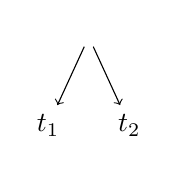
\begin{tikzpicture}
			      \node(A){};
			      \node(B)[below=of A, yshift=-1cm, left=0.25cm]{$t_1$};
			      \node(C)[below=of A, yshift=-1cm, right=0.25cm]{$t_2$};

			      \draw[->] (A) -- (B);
			      \draw[->] (A) -- (C);
		      \end{tikzpicture}
		\item And no other trees.
	\end{enumerate}
\end{definition}

\subsection{Encodings in $\mathbb{D}$}
\subsubsection{Lists}
\begin{definition}
	The empty list is encoded as the empty tree $nil$.

	Appending an element to the front is modelled by $<\_.\_>$.

	$$\enc{[]}=nil$$

	$$\enc{[a_1,a_2,\ldots,a_n]}=<\enc{a_1}.<\enc{a_2}.<\ldots<\enc{a_n}.nil>>>>$$

	$$\enc{[[],[]]}=<nil.<nil.nil>>$$

	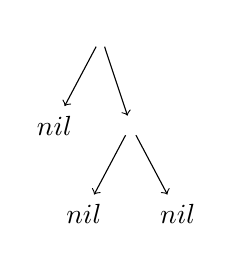
\begin{tikzpicture}
		\node(N){};
		\node(L)[below=of N, yshift=-1cm, left=0.25cm]{$nil$};
		\node(R)[below=of N, yshift=-1cm, right=0.25cm]{};
		\node(RL)[below=of R, yshift=-1cm, left=0.25cm]{$nil$};
		\node(RR)[below=of R, yshift=-1cm, right=0.25cm]{$nil$};

		\draw[->] (N) -- (L);
		\draw[->] (N) -- (R);
		\draw[->] (R) -- (RL);
		\draw[->] (R) -- (RR);
	\end{tikzpicture}
\end{definition}

Notice how the nil tree drawing has a \textit{spine}, ending in a $nil$ terminator.

\subsubsection{Booleans}
\begin{definition}
	$$\enc{false}=nil$$
	$$\enc{true} = <nil.nil>$$
\end{definition}

\subsubsection{Numbers}
\begin{definition}
	$$\enc{0} = nil$$
	$$\enc{n+1}=<nil.\enc{n}>$$
\end{definition}

Thus numbers are effectively defined as a list of $n$ $nil$s.

\subsection{While language semantics}
$$\llbracket \_ \rrbracket^{while}:\mathbb{D}\mapsto{\mathbb{D}_\bot}$$

\begin{figure}[H]
	\begin{lstlisting}[frame=single]
prog p read X { ... } write Y
\end{lstlisting}
	\captionof{lstlisting}{$\llbracket p \rrbracket^{while}(X)=Y$}
\end{figure}

\begin{figure}[H]
	\begin{equation}
		\llbracket q \rrbracket^{while}(d)=\bot
	\end{equation}
	\captionof{figure}{Implying that program $q$ does not terminate.}
\end{figure}

\subsection{Stores}
\begin{definition}
	A store is a key value pair set. A framework for variables in our programs.

	$$\{x_1:d_1,\ldots,x_n:d_n\}$$

	A store has a set of operations that must be defined on it.
	\begin{itemize}
		\item Lookup $x$: $\sigma(x)$.
		\item Update $x$ to $d$: $\sigma[x:=d]=\sigma | \{(x,val)\}\cup\{x,d\}$
		\item Initial store for $d$: $\sigma_0^p(d)=\{x:d\}$, other variables are implicitly assigned $nil$.
	\end{itemize}
\end{definition}

\subsection{Semantics of commands}
$$s\vdash\sigma_1\to\sigma_2$$
i.e. a statement list $s$ takes store $\sigma_1$ and yields $\sigma_2$.

Thus,

\begin{figure}[H]
	\begin{lstlisting}
  p read X { S } write Y
  \end{lstlisting}
	\begin{equation}
		\llbracket p \rrbracket^{while}(d)=
		\begin{cases}
			e    & \textrm{if }s\vdash\sigma_o^p(d)\to\sigma \textrm{ and } \sigma(Y)=e \\
			\bot & \textrm{otherwise}
		\end{cases}
	\end{equation}
\end{figure}

\subsection{Core while and extensions}
The core while language has:
\begin{itemize}
	\item No test for equality
	\item No procedures or macros
	\item No literals
	\item No built in list notation
	\item No switch case
	\item Only one atom ($nil$)
\end{itemize}

Not having these features makes it more difficult to program.
Not impossible, just more difficult / tedious.

\subsubsection{Macro calls}
Macro calls are an interesting case.

In most modern languages, calling an externally defined function would execute said function
in a scope lower than that of the caller's scope, this is not the case in while.

While has no concept of scopes, calling a macro literally results in copying the instructions
of the macro into the position of the call. This means that variables used in the macro
will affect and be accessible from the caller's context.

Therefore one must think carefully when creating macros in while.

\section{Programs as data objects}
If $L$ has `Programs as data`, we can write compilers, interpreters, and specialisers in $L$.

$L$ has `Programs as data` if $L$-data permits the encoding of $L$-programs.

$L$ has `pairing` if $L$-data permits encoding pairs of objects.

\begin{definition}
	\textbf{Program specialiser}
	A program which takes a program with two inputs and one data, and partially evaluates that program.
\end{definition}

While can have `Programs in data`, we must just define the encoding of a program into a binary tree.

\begin{definition}
	\textbf{Interpreter}
	Given a language $S$, where $\mathbb{D}_S\subseteq\mathbb{D}_L$, an interpreter
	$int$ in $L$ which interprets $S$ must fulfill:

	$$\llbracket int \rrbracket^L(\enc{p}, d)=\llbracket p \rrbracket^S(d)$$
\end{definition}

\part{Complexity}
\section{Measuring Time Usage}

\begin{definition}
	\textbf{Unit-cost time measure}
	For an imperative language $L$, the function $time^L:L_{program}\to L_{data}\to\mathbb{N}_\bot$ is defined as follows:
	For any $p\in L_{program}$, and $d\in L_{data}$ we define

	$$
		time^L_p(d)=
		\begin{cases}
			t+1  & \textrm{ if }p\vdash s_1\to s_2\ldots\to s_t \textrm{ where } s_1=readin(d) \textrm{ and } s_t \textrm{ terminal} \\
			\bot & \textrm{otherwise}
		\end{cases}
	$$
\end{definition}

This is effectively a definition of basic steps in the program. The idea is that if a program
consisting of $t$ unit steps terminates, we can give its unit-cost execution time as $t+1$.

Notably the read input and write output is implicitly one step each.

This function also captures the idea that the running time depends on the input data $d$.

Is this model fair? It doesn't necessarily account for complex expressions like equality in while,
or unbounded number size in registers under the RAM model. Given this, we may apply the Unit-cost
time measure to TM, GOTO, and CM models, but not to while, SRAM, RAM.

\subsection{Measuring in RAM \& CM}

\part{The hardness of problems}
\section{Rice's Theorem}
\begin{definition}
	\textbf{Rice's Theorem}

	All non-trivial and extensional properties of programs are undecidable.
\end{definition}

\section{The Halting Problem}

Note the following notation:

$f:\mathbb{D}\mapsto\mathbb{D}_\bot$ is while computable if there is
some $p$ such that $f=\llbracket p \rrbracket^{while}$

$f(d)=\bot$, $f$ is undefined at $d$.

$f(a)\downarrow$, $f$ is defined at $a$.

A set $\textbf{A}\subseteq \mathbb{D}$ is while-decidable if there is
$\llbracket p \rrbracket^{while}(d)\downarrow$ for all $d\in\mathbb{D}$, and $d\in A$ if and only if
$\llbracket p \rrbracket^{while}(d)\downarrow$ is true.

$[p,d]$ is a while program $p$ as data.
\begin{definition}
	\textbf{The Halting Problem}

	$$HALT\subseteq\mathbb{D} = \{[p,d]\in\mathbb{D}|\llbracket p \rrbracket^{while}(d)\downarrow\}$$

	in other words, $HALT$ is the set of all programs-as-data which are defined
	for some $d\in\mathbb{D}$. i.e. does some program $p$ terminate for an input $d$.
\end{definition}

We can prove that the Halting problem is undecidable by contradiction.

Suppose that some $h$ exists which solves the halting problem. i.e. $h$ is a program
which examines another program and returns true if it terminates, and false if it doesnt:

\begin{lstlisting}
h read A { B } write C
\end{lstlisting}

We then create another program $r$:

\begin{lstlisting}
r read X {
  A := [X, X];
  B;
  Y := C
  while (Y) { Y := Y; }
} write Y
\end{lstlisting}

Is it then true that $\llbracket r \rrbracket(r)\downarrow$ holds?

We get $C=\llbracket h \rrbracket^{while}[r,r] = Y$

If $Y$ is true, i.e. if $h$ says that $r$ will terminate, then $r$ will never terminate,
but if $h$ says that $r$ will not terminate, then $r$ will terminate.

This is a contradiction, proving that the halting problem is not decidable
in the while language.

The technique used in this proof is the Barber Paradox technique, basically asking does $X$ hold with input $X$.

\subsection{While semi-decidability}
\begin{definition}
	\textbf{While Semi-Decidability}
	A set $A\in\mathbb{D}$ is While semi-decidable if and only if, there exists a while program $p$ such that for all
	$d\in\mathbb{D}$, the following holds: $d\in A$ if and only if $\llbracket p \rrbracket^{while}(d) = true$.
\end{definition}

The halting problem is while semi-decidable, this is proven with the following.
\begin{lstlisting}
sd read PD {
  Res := <u> PD;
  X := true
} write X
\end{lstlisting}

For this program, any input in $\mathbb{D}$ yields $true$.

\begin{definition}
	\textbf{Decidability}
	\begin{enumerate}
		\item Any finite set $A\subseteq\mathbb{D}$ is while-decidable.
		\item If $A\subseteq\mathbb{D}$ is while decidable, then so is its complement in $\mathbb{D}$.
		\item Any while decidable set is while semi-decidable.
		\item A problem (set) $A\in\mathbb{D}$ is while decidable if and only if, both $A$ and its complement
		      $\mathbb{D}\\A$ are while semi-decidable.
	\end{enumerate}
\end{definition}

\begin{definition}
	\textbf{`Interesting` properties of programs}
	An `interesting` property is both \textbf{non-trivial} and \textbf{extensional}.

	\begin{itemize}
		\item \textbf{non-trivial} properties are those which not all programs have, but at least one program has.
		\item \textbf{Extensional} properties are those which depend on the input / output behaviour of the program,
		      i.e. its' semantics.
	\end{itemize}

	Formally, a property $A$ is a subset of while programs.

	\begin{itemize}
		\item $A$ is \textbf{non-trivial} if $\{\}\neq A\neq \textrm{while-programs}$.
		\item $A$ is \textbf{extensional} if for all $p,q\in\textrm{while-programs}$ such that
		      $\llbracket p\rrbracket^{while}=\llbracket q \rrbracket^{while}$ it holds that $p\in A$ if and only if $q\in A$.
	\end{itemize}

\end{definition}

With this knowledge, we can prove Rice's theorem by contradiction. Assume $A$ is decidable, we must then show that
the Halting problem is decidable.

\begin{figure}[H]
	\begin{lstlisting}
diverge read X {
  while true {}
} write Y
\end{lstlisting}
	$\llbracket diverge \rrbracket^{while}(d)=\bot$ for any $d\in\mathbb{D}$.
\end{figure}

Now let us assume that $diverge\in A$. By the non-triviality of $A$, we know that there is a program not in $A$.
Let us call this program $comp$. $comp\notin A$.

\begin{lstlisting}
q read X {
  Y := <p> "e";
  Res := <comp> X
} write Res
\end{lstlisting}

Consider the behaviour of $q$. If $\llbracket p \rrbracket^{while}(e)=\bot$, then clearly
$\llbracket q \rrbracket^{while}(d)=\bot$ for all $d\in\mathbb{D}$. But if $\llbracket p \rrbracket^{while}(e)\downarrow$,
then $\llbracket q \rrbracket^{while}(d)=\llbracket comp \rrbracket^{while}(d)$ for all $d\in\mathbb{D}$.

\begin{equation}
	\llbracket q \rrbracket^{while}=\begin{cases}
		\llbracket diverge \rrbracket^{while} & \textrm{if }\llbracket p \rrbracket^{while}(e)=\bot     \\
		\llbracket comp \rrbracket^{while}    & \textrm{if } \llbracket p \rrbracket^{while}(e)\neq\bot
	\end{cases}
\end{equation}

Which implies that $diverge\in A$ iff $q\in A$, if $\llbracket p \rrbracket^{while}(e)=\bot$,
and $comp\in A$ iff $q\notin A$ if $\llbracket p \rrbracket^{while}(e)\neq\bot$.

We know $diverge\in A$ and $comp\notin A$, because of our initial assumptions. Which means that if
we can decide $A$, then we can decide the Halting problem, since $A$ is an extensional property,
and the Halting problem is about an extensional property of a program.

This is a contradiction, and we can therefore conclude that Rice's theorem is correct.

\section{$\mathbb{P}$ and $\mathbb{NP}$}
A problem is in $\mathbb P$ if it can be solved in polynomial time. A problem is in $\mathbb{NP}$
if it \textit{cannot} be solved in polynomial time or better, but you can write a verifier for said problem
which runs in polynomial time.

\begin{definition}
	\textbf{Verifier}
	A Verifier takes a candidate solution to a problem (the certificate), and
	`verifies` whether or not it is actually a valid solution.

	A Verifier should also define a quality measure $k$, the result of the program
	being determined by whether or not $k$ is higher than some threshold.
\end{definition}

One may also determine if a problem is in $\np$ using a non-deterministic Turing Machine.

$A\in\np$ if and only if $A$ is accepted by a non-deterministic Turing Machine with Polynomial time bound.

One may introduce non-determinism into the Turing Machine model with:
$\mathcal{L}:\textrm{goto }\mathcal{L}'\textrm{ or }\mathcal{L}''$. In such a model, semantics is no longer
a function but a relation, relating an input to a set of possible outputs.

$p$ accepts $d$ if $(d, true)\in\llbracket p \rrbracket ^L$.

One can prove that $\p\subseteq\np$, since problems in $\p$ clearly have a polynomial time verifier,
i.e. the same program that provides solutions in polynomial time can serve as a polynomial time verifier.


\end{document}
